
%
% conclusions
%

\chapter{Conclusions \& outlook}
\label{chapter:conclusions-outlook}

\section{Performance evaluation}
\label{chapter:performance}

Performant real-time clustering is the main objective of this thesis as formulated in chapter \ref{chapter:objective-performance}. As a requirement, the algorithm should cluster in real-time to support dynamic queries and cluster up to 1,000,000 items within less than one second.

The configuration of the demo use case implementation described in chapter \ref{chapter:use-case-demo} was used to do automated performance testing of the different clustering algorithms. A \textit{Bash}\footnote{\url{http://en.wikipedia.org/wiki/Bash\_(Unix\_shell)}} script was created to test the performance of the clustering algorithm based against an incrementing number of items.

\begin{figure}[h]
  \begin{center}
    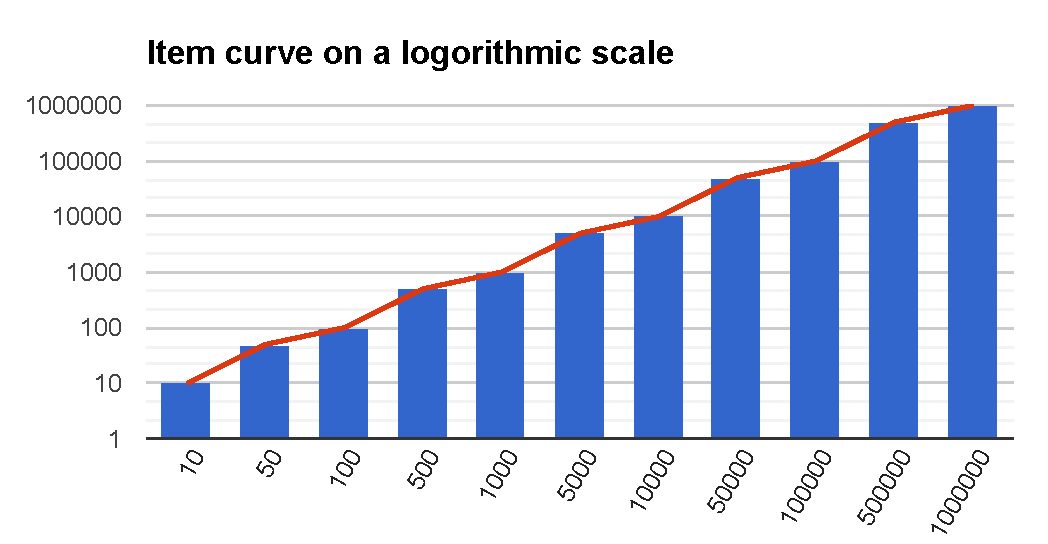
\includegraphics[width=0.8\textwidth]{figures/performance_items.pdf}
    \caption{Item curve on a logorithmic scale.}
    \label{fig:performance-items}
  \end{center}
\end{figure}

The script exponentially increases items to test the clustering performance from a base 10 up to 1,000,000 items. Between every two steps of the exponential function, an intermediary step of the half of the two steps will be inserted. While the exponential mean value for example between 100 and 1000 items would be 316.2, this approach inserts 500 to improve readability of the results for humans. The resulting curve of items tested is visualized in figure \ref{fig:performance-items}.

The \textit{ab} command of the ApacheBench\footnote{\url{http://en.wikipedia.org/wiki/ApacheBench}} is used to sequentially repeat the same requests and calculate a mean response time value. Hereby the script tries to circumvent variations caused by external factors as the server hardware and operating system.

The results of the performance benchmark have been extracted and aggregated into a chart as show in figure \ref{fig:algorithm-performance}. It is clearly shown that that the three implemented algorithms perform very differently. Each algorithm scales up to a certain number of items, while beyond this threshold, performance decreases significantly. The PHP-based clustering algorithm is very limited in such that requests for up to 1,000 clustered items can be completed within one second. The MySQL-based clustering approach scales much better but requests get slow beyond 100,000 items. The most performant algorithm implementation is the Solr-based one that server 1,000,000 items still in a reasonable amount of time. 

\begin{figure}[h]
  \begin{center}
    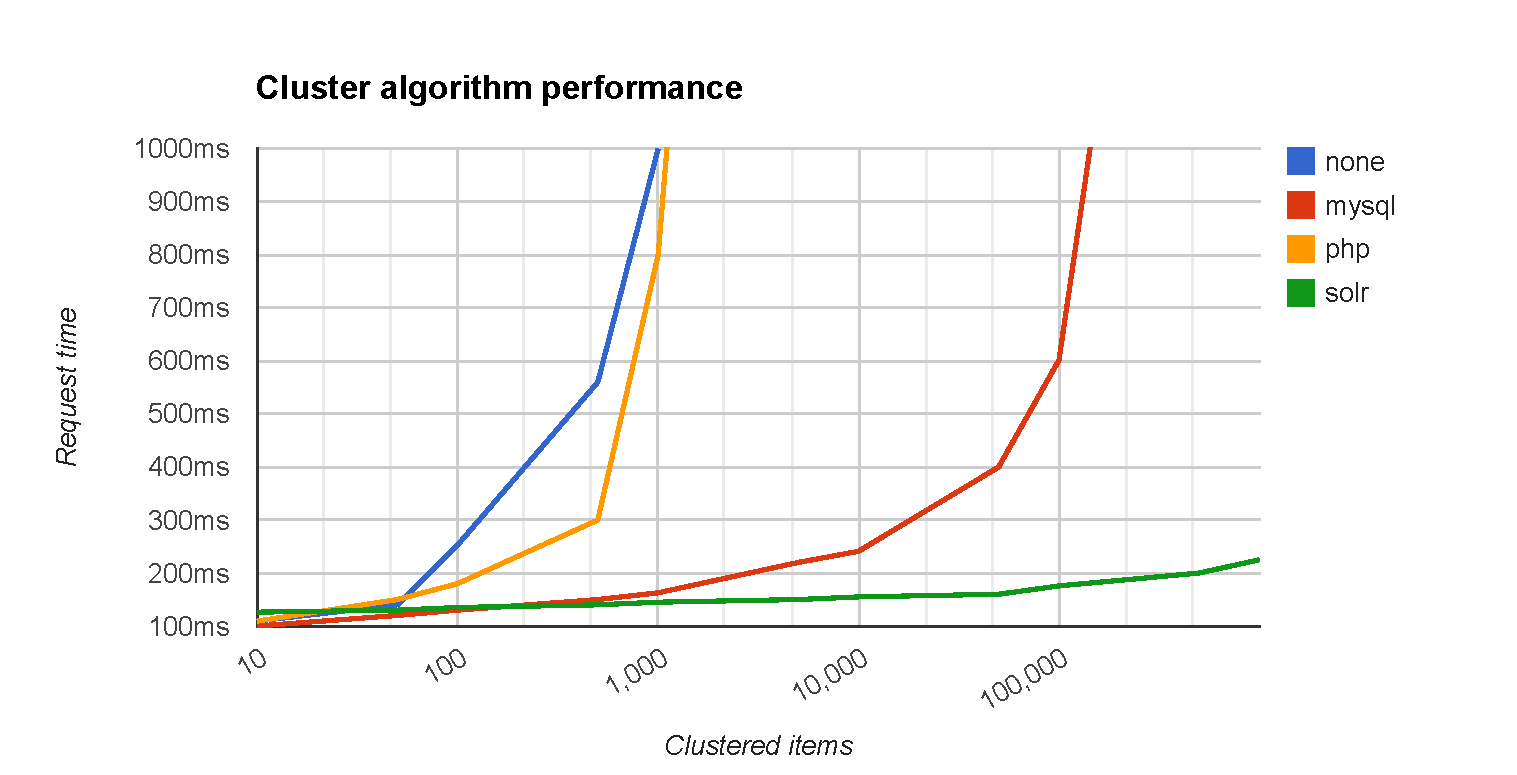
\includegraphics[width=1.2\textwidth]{figures/geocluster_algorithm_performance.pdf}
    \caption{Geocluster performance in milliseconds per algorithm and number of items.}
    \label{fig:algorithm-performance}
  \end{center}
\end{figure}

A deeper analysis of the PHP-based algorithm clearly shows that the most time-consuming part of the algorithm is creating the clusters based on Geohash. As all unclustered items need to processed after executing the database query have to be processed, this part takes the most time. In an example based on a query with 9270 items, the entire roundtrip between client and server takes 26.71 seconds. Querying the items just took 100ms. With 24.32 seconds, the Geohash-based pre-clustering consumes the major part of the execution time. For the same amount of items, a request using the MySQL-based algorithm was completed within 194 ms. In this case, the query was completed after 80 ms and the while clustering process was finished 8 ms seconds later. The remainder of the processing time was consumed by Drupal performing non-clustering related processing before and at the end of the request. This example shows, how shifting the main clustering task into the database can increase performance for a certain range of number of items. As stated before, when approaching 100,000 items the MySQL-based algorithm is getting significantly slower, as the query itself takes longer.

Given the numbers, the performance criterion of this thesis could be fulfilled. While the PHP-based implementation isn't really usable, MySQL-based and Solr-based clustering can be used to create performant, interactive maps with Drupal for item sets up to at least 1,000,000 items. While we know that MySQL-based clustering only scales up to 100,000 items, the threshold for Solr-based clustering wasn't determined as tests were limited up to 1,000,000 items. It is expected that there is room for improvements and optimizations for all of the algorithms.

Another performance-related aspect is cachability of responses and results. Apache Solr and Drupal itself already incorporate various caching layers. Caching clustered results for the server-side clustering solution mainly depends on the parameters of the Bounding Box strategy. As currently, every minor change to the bounding box will issue a different request to the server, these can't be cached efficiently. A possible solution discussed\footnote{\url{http://drupal.org/node/1868982}} is to define granular steps for the bounding box in order to produce repeating requests that can be cached.  

\section{Further evaluation}

The second objective on integration and extensibility defined in chapter \ref{chapter:objective-integration} has been fulfilled by the Geocluster module as it integrates with Views, Views GeoJSON and other Drupal mapping modules. In addition, the implementation of the clustering algorithm can be extended using plugins as explained in chapter \ref{chapter:impl-alg}. Geocluster was also released under the GPL license as required by objective \ref{chapter:open-source}. With regards to objective \ref{chapter:objective-use-cases}, a demo use case has been implemented that show cases all the functionality needed. The actual GeoRecruiter use case hasn't been implemented, but as stated in \ref{chapter:use-case-georecruiter}, the groundwork has been established in order to do so. Finally, main usability concerns have been realized with the Geocluster Visualization component.

While most objectives have been reached, there are still many parts of the Geocluster implementation that can be improved upon:

\begin{itemize}

\item \textbf{Cluster sizes}: The current implementation doesn't respect the size of a cluster. As naturally, a cluster with more items can be visualized larger than smaller clusters, the algorithm could be improved for growing clusters by their size. The bigger size of a cluster would therefore reduce the distance to its neighbor clusters, potentially merging additional neighbors into it. Andrew Betts describes a similar approach under the term \textit{``Grid based viral growth argorithm''}\footnote{\url{http://web.archive.org/web/20071121140547/http://trib.tv/tech/clustering-points-on-a-google-map/}}.

\item \textbf{Cluster centers}: While the PHP- and MySQL-based algorithm provide means of calculating a centroid as the center of a cluster, the Solr-based clustering algorithm is limited in this regards. Solr doesn't seem to provide the same functionality to calculate the mean value for a field using the grouping function, as the MySQL-based algorithm leverages the $AVG$ function for latitude and longitude. Potentially, the stats component\footnote{\url{http://wiki.apache.org/solr/StatsComponent}} could be used for calculating the centroid of cluster items within the Solr-based algorithm.

\item \textbf{Processing clustered results}: The way that the Drupal mapping stack integrates with the Views module isn't designed for processing clustered results. The current implementation of Geocluster performs various workarounds in order to inject clustered results into the process. Especially for the Solr-based implementation this leads to code-duplication because in the standard case results are processed as arrays while in the other case, results need to be PHP objects. If possible, a cleaner way of integrating clustering with the related modules is desirable.   

\item \textbf{Improve client-side handling and visualization}: The current implementation for visualizing clustered results is very basic. A relative sizing of cluster items according to their clusters is needed and should also be supported by the algorithm as stated before. In addition, it would be good to have be a clean way to configre the how data for clustered results should be displayed and integrate it with how non-clustered data is represented. For low zoom levels, the roundtrip to the server for fetching a separate clustered result on every bounding box change can be an overhead. Christopher Calid\footnote{\url{http://drupal.org/user/210499}} proposed a way of ``Progressively enhance server-side with client-side clustering''\footnote{\url{http://drupal.org/node/1914704}}. The intention is to transition from server-side clustering higher zoom levels to client-side clustering for lower zoom levels.

\end{itemize}

\section{Conclusions}

Writing this thesis and implementing Geocluster was basically a process of over one year. Before starting the thesis, I conducted a research project named AustroFeedr\footnote{\url{http://www.austrofeedr.at/}} on real-time processing technologies for aggregating, processing and visualizing data with Drupal. One main aspect of AustroFeedr was a Drupal-based visualization component using OpenLayers maps. After I had completed AustroFeedr by the end of 2011, I researched Drupal and mapping related topics for writing this master thesis in Software Engineering \& Internet Computing at Technical University Vienna.

The topic server-side clustering for Drupal was decided upon thanks to recommendation by Th\'eodore Biadala\footnote{\url{http://drupal.org/user/598310}}, an active JavaScript and maps contributor in the Drupal community who I met at the Frontend United conference in Amsterdam, April 20-22. After doing some initial research and prototyping, I organized a mapping sprint at Drupal Developer Days Barclona\footnote{\url{http://groups.drupal.org/node/234168}}. This is where Nick Veenhof\footnote{\url{http://drupal.org/user/122682}}, active Apache Solr contributor within the Drupal community, came up with the idea of researching Geohash for realizing an efficient clustering algorithm.

It took until September 2012, when I implemented a first prototype of the PHP-based clustering algorithm and figured out basic integration needs for to make the clustering task work with Drupal. From then, several iterations and alpha releases of Geocluster led to completing MySQL and Solr-based clustering by the end of 2012. As by finishing this thesis in March 2013, performance tests have been concluded for Geocluster and a first beta release has been published.

There has already been some positive feedback from people interested in using Geocluster as a drop-in solution to create scalable maps using server-side clustering. On the other hand, I have to admit that integration clustering into a complex stack such as the Drupal mapping stack has its advantages and disadvantages. Geocluster does a decent job at clustering data server-side, but the tight integration into the Drupal stack also comes at the cost of overhead and complex integration code. Given the expertise in writing code, it can make sense to create a custom server-side clustering solution for a specific purpose without depending on a number of separate modules. Still, the generic approach has the benefit of others potentially being able to use the Geocluster module. Writing this thesis was both challenging and fun. Working on something and being able to share it with the Drupal community, a steadily growing team of contributors of Free and Open Source software, has been a rewarding experience and a solid source of motivation. 

\section{Future work}

Direct community feedback and indirect indicators like the project usage statistics will show if and how the Geocluster module is used by others. As stated before, there are many implementation details that can be enhanced. At epiqo, we are planning to incorporate Geocluster for location-based searches of large-scale job portals based on the Recruiter distribution as stated in chapter \ref{chapter:use-case-georecruiter}. 

Thanks to a scholarship by the Drupal association, I will be able to attend DrupalCon Portland\footnote{\url{http://portland2013.drupal.org/}}. Together with other Drupal mapping contributors, we have proposed a panel discussion\footnote{\url{http://portland2013.drupal.org/session/should-have-made-left-turn-albuquerque-panel-discussion-challenges-buildingincorporating}} which would be a great opportunity to discuss server-side clustering as one strategy for creating scalable, interactive maps with Drupal.

